\section{IMPLEMENTATION DETAILS}
\subsection{Preprocessing}

Before training the model, we preprocess the dataset as follows:

\subsubsection{Resize}
All images, whether sourced from videos or other datasets, were resized to a consistent resolution of 256x256 pixels. This resizing ensured a uniform input size for the vision transformer.

\begin{figure}[ht]
    \centering
    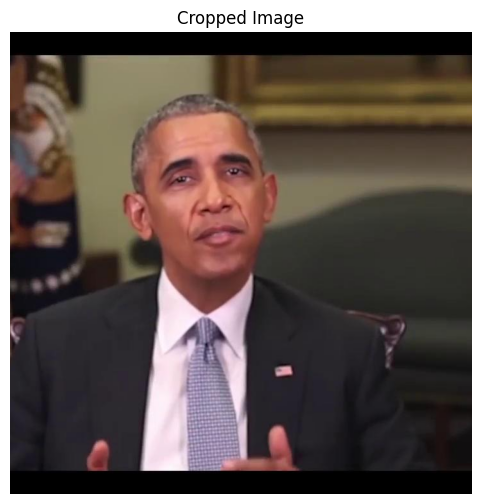
\includegraphics[width=2in]{img/cropped.png}
    \caption{Cropped Image}
    \label{fig:cropped}
\end{figure}

\begin{figure}[ht]
    \centering
    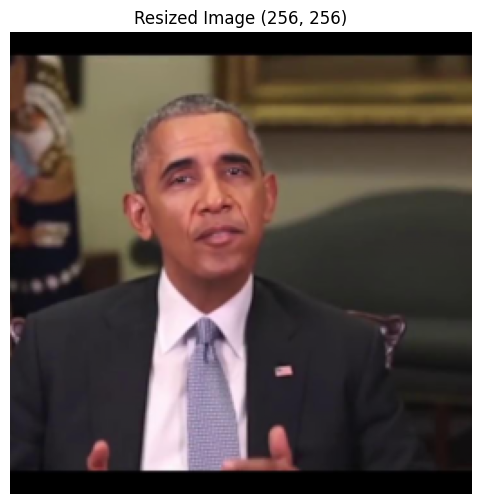
\includegraphics[width=2in]{img/resized.png}
    \caption{Resized Image}
    \label{fig:resized}
\end{figure}

\subsubsection{Augmentation} To increase the dataset's diversity and improve the model's ability to generalize, we applied various data augmentation techniques. These techniques included random rotations, horizontal flips, brightness adjustments, and minor deformations.
\newpage
\subsubsection{Normalization} Pixel values of the images were normalized to a specific range to ensure consistent input for the model during training and inference.

\begin{figure}[htbp]
    \centering
    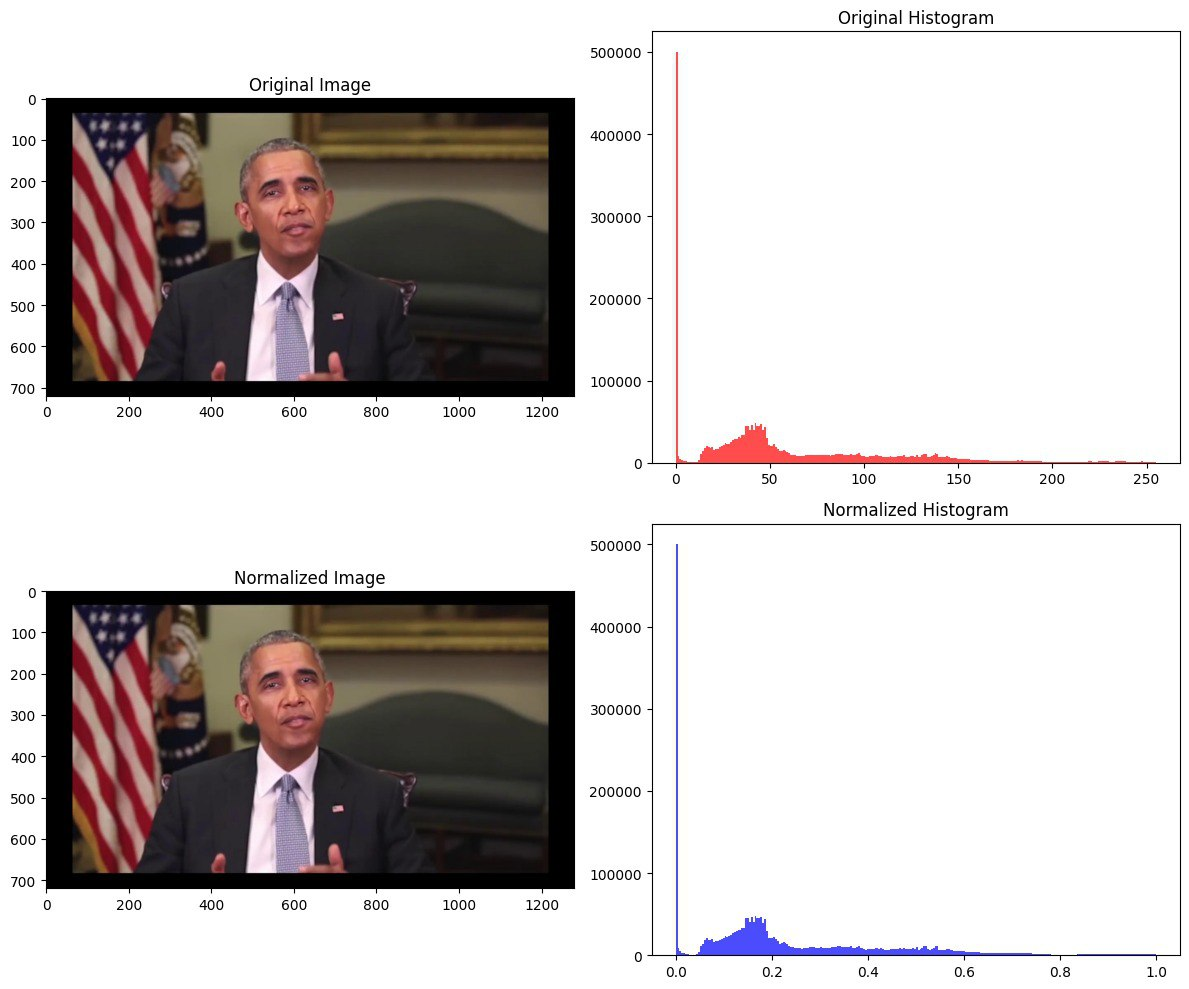
\includegraphics[width=5in]{img/normalized.jpg}
    \caption{Normalization}
\end{figure}

By preprocessing the dataset, we enhanced the model's capacity to learn relevant features and intricate patterns required for accurate deepfake detection.
\newpage

\subsection{Face Alignment Integration}

The Face Alignment library plays a pivotal role in our system, contributing essential capabilities for precise face detection and facial feature extraction. The integration of Face Alignment enhances the accuracy of our system by ensuring optimal alignment of facial features during the analysis process.

\subsubsection{Working Principle}

\begin{enumerate}
    \item \textbf{Landmark Detection:} Face Alignment detects facial landmarks, such as eyes, nose, and mouth, serving as anchor points for accurate alignment and feature extraction.

    \item \textbf{Face Localization:} Advanced algorithms are used to locate and identify the face within an image, determining the bounding box or region of interest containing facial features.

    \item \textbf{Affine Transformation:} Facial landmarks are aligned using affine transformation techniques, ensuring consistent positioning of features across different images.


\end{enumerate}

\begin{figure}[htbp]
    \centering
    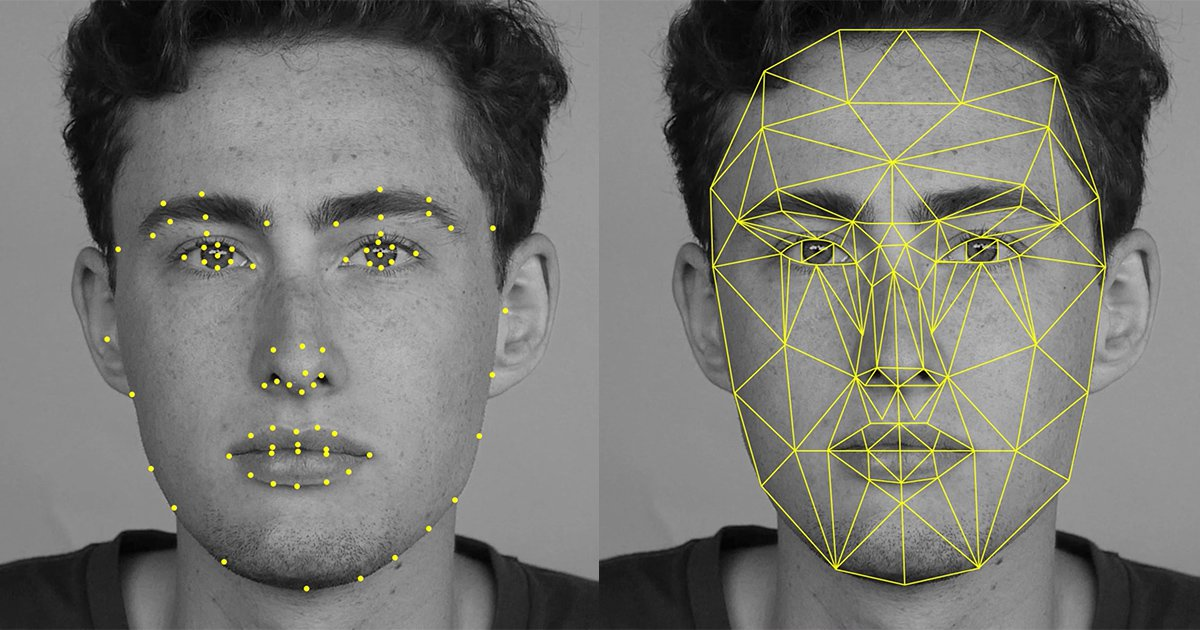
\includegraphics[width=5in]{img/facial feature.jpg}
    \caption{Facial Landmark Detection}
\end{figure}

By incorporating the Face Alignment library into our project, we ensure that facial features are consistently and accurately represented, thereby enhancing the overall performance of DefaceLab in detecting manipulated or fake media.

\newpage